\chapter{Arquitetura de Software do~\textit{JOGUE-ME}}\label{chapter:arquitetura_captura}

A arquitetura do sistema possui diferentes tecnologias conforme a Figura~\ref{fig:arquitetura} e foi desenvolvida para permitir o desenvolvedor abstrair da complexidade do processamento do sinal dos dados e na identificação dos sintomas motores. Logo, esta arquitetura de \textit{software} integrada a uma \textit{engine} de jogos bem conhecida e difundida (Unity 3D~\cite{unity3d}) facilita o desenvolvimento de jogos para esse contexto.

%A arquitetura desenvolvida para o~\ac{jogue-me} busca abstrair das dificuldades existentes no desenvolvimento de um jogo para monitoramento de dados de saúde. Neste projeto foi desenvolvido um arcabouço de software, integrado a uma \textit{engine} de jogos bem difundida e utilizada por desenvolvedores de jogos. Devido a essa estrutura, buscamos facilitar a programação de jogos para a saúde, criando Componentes de \textit{Software} sobre a \textit{engine} de jogos Unity 3D~\cite{unity3d}. Assim, desenvolvedores de jogos podem criar \text{JOGUE-MEs}, usando esse arcabouço (Seção~\ref{sec:cliente_game}), o que permite ao desenvolvedor encapsular os aspectos de processamento de sinal. 


\begin{figure}[!h]
 \centering
  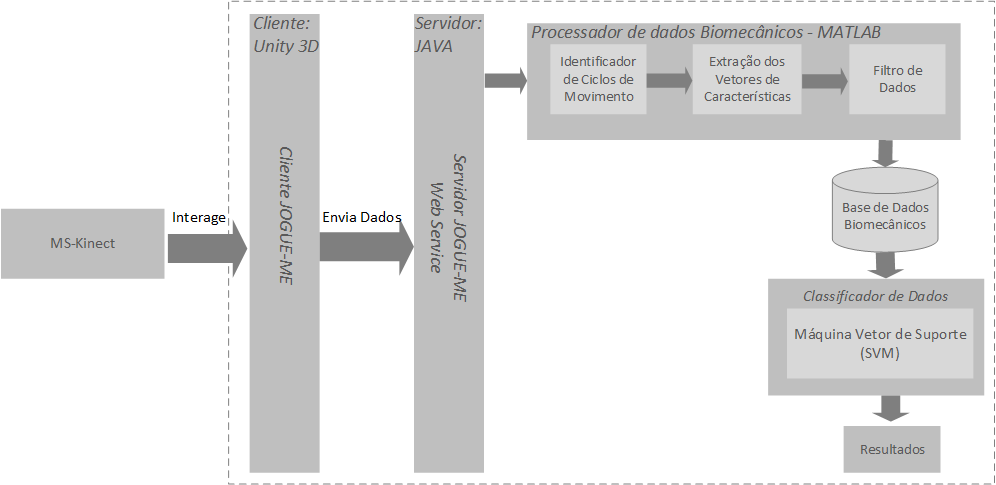
\includegraphics[scale=0.56]{./img/arquitetura.png}
 % matrixargseg.png: 296x162 pixel, 100dpi, 7.52x4.11 cm, bb=0 0 213 117
 %\caption{Estágio desenvolvimento de jogos ~\cite{fullerton2008game}}
\caption[Arquitetura de Software]{Arquitetura de Software}
%  \caption{Estágio desenvolvimento de jogos}
 \label{fig:arquitetura}
\end{figure}

\section{Arquitetura do ~\textit{JOGUE-ME}}\label{sec:cliente_game}
A arquitetura do~\ac{jogue-me} para o desenvolvimento de jogos utiliza uma \textit{engine} de jogos (Unity3D~\cite{unity3d}), que é um ambiente de desenvolvimento de jogos multi-plataforma. Esta \textit{engine} possibilita que os desenvolvedores abstraiam-se dos aspectos de hardware, plataforma e complexidade do desenvolvimento de jogos e habilita o desenvolvedor a se ater somente às atividades referentes ao desenvolvimento do jogo.

Atualmente, desenvolvedores independentes de jogos utilizam Unity3D~\cite{unity3d} como ferramenta de desenvolvimento. Esse ambiente facilita a criação de cenários, terrenos e interação com os objetos dos jogos usando uma linguagem de \textit{script}. No entanto, desenvolver jogos com propósito de monitorar sinais motores possui desafios que não precisam ser de responsabilidade dos desenvolvedores de jogos. Por esse motivo, criamos uma arquitetura de software para o cliente JOGUE-ME (Figura~\ref{fig:arquitetura_cliente}) que abstrai a complexidade do desenvolvimento de um jogo de monitoramento da saúde.

\begin{figure}[!htbp]
 \centering
 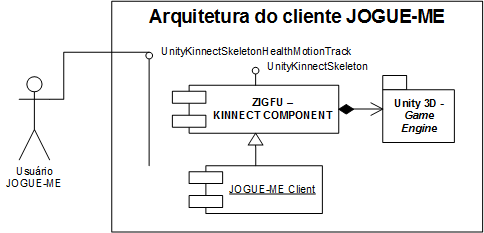
\includegraphics[scale=0.8]{./img/arquiclientejogueme.png}
 % matrixargseg.png: 296x162 pixel, 100dpi, 7.52x4.11 cm, bb=0 0 213 117
 %\caption{Estágio desenvolvimento de jogos ~\cite{fullerton2008game}}
\caption{Arquitetura JOGUE-ME: Módulo Cliente de Aquisição de Sinais Motores}
%  \caption{Estágio desenvolvimento de jogos}
 \label{fig:arquitetura_cliente}
\end{figure}


Para adquirir os sinais motores, este trabalho utilizou e herdou do componente (Zigfu~\cite{zigfu}) para Unity3D para integrar o Ms-Kinnect~\cite{kinnect2013} como controlador do jogo à arquitetura proposta. O Ms-Kinnect~\cite{kinnect2013} é um sensor de captura de movimentos utilizado tanto para o console MS-XBOX 360 quanto para \textit{PCs}. Ele permite a aquisição dos sinais relativos ao movimento humano e identifica as articulações por meio da posição anatômica do corpo humano~\cite{hamill1999bases}.
%, como pode ser visto na Figura~\ref{fig:articulacoeskinnect}.



%Os jogos eletrônicos que fazem uso dos movimentos do corpo permitem a liberdade de movimento, logo o movimento exercido nestes possibilitam muita variabilidade. Logo, é necessário que o desenvolvedor tenha a informação de quais ações o jogador precisa executar para que estas sejam monitoráveis. As ações de um~\ac{jogue-me} devem estar descritas no~\ac{jogue-me}(Seção~\ref{subsec:game_actions_guide}) como estabelecido no processo de desenvolvimento proposto no Capítulo~\ref{chap:processo_desenvolvimento}.


%\begin{figure}[!htbp]
 %\centering
 %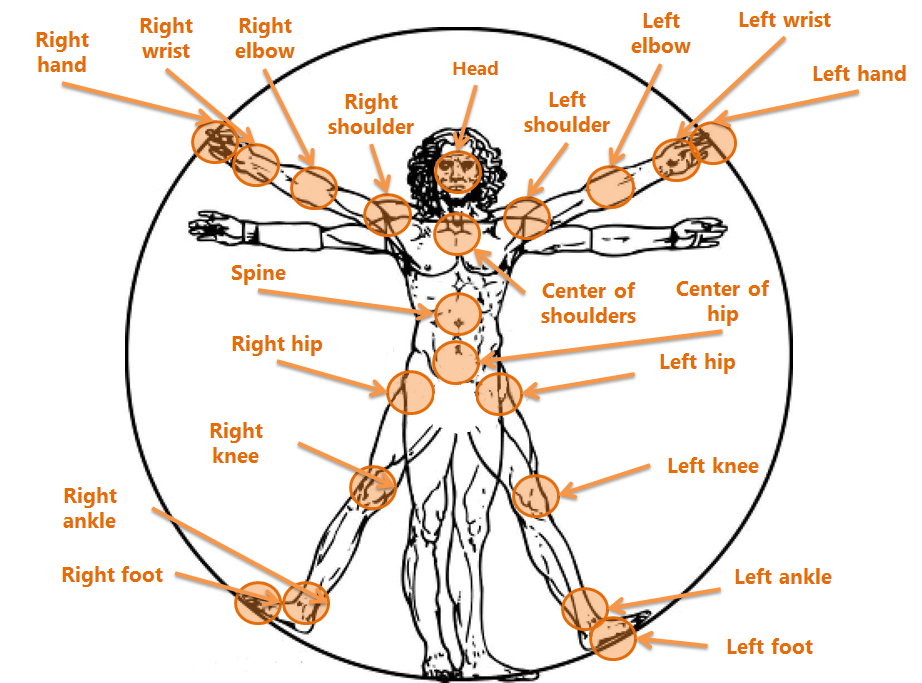
\includegraphics[scale=0.4]{./img/articulacoes.png}
 %% matrixargseg.png: 296x162 pixel, 100dpi, 7.52x4.11 cm, bb=0 0 213 117
 %%\caption{Estágio desenvolvimento de jogos ~\cite{fullerton2008game}}
%\caption[Posições das Articulações do Corpo Humano Adquiridas Pelo MS-Kinnect]{\copyright Posições das Articulações do Corpo Humano Adquiridas Pelo MS-Kinnect ~\cite{kinnect2013}}
%%  \caption{Estágio desenvolvimento de jogos}
 %\label{fig:articulacoeskinnect}
%\end{figure}
\begin{figure}[!h]
 \centering
 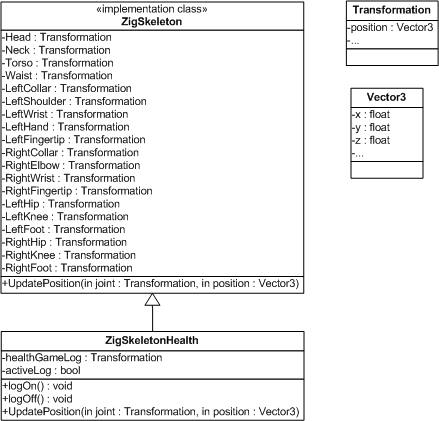
\includegraphics[scale=0.8]{./img/diagclasszigfu.png}
 \caption{Diagrama de Classe do ZigSkeleton e ZigSkeletonHealth}
 \label{fig:diagramaclassezigfu}
\end{figure}

O Zigfu ~\cite{zigfu} é um componente de software que permite integrar o Ms-Kinnect ao Unity3D. O Zigfu faz um mapeamento das articulações adquiridas pelo Ms-Kinnect, para uma classe chamada \textit{ZigSkeleton}, com todas as articulações, como podemos ver no Diagrama de Classe (Figura~\ref{fig:diagramaclassezigfu}). No entanto, para adquirir os sinais motores, é necessário armazenar os valores das posições das articulações durante as ações dos usuários. Por esse motivo, o Zigfu foi extendido na classe \textit{ZigSkeletonHealth} para armazenar as posições das articulações, além de um mecanismo para habilitar ou desabilitar o monitoramento dos sinais (métodos \textit{logOn() e logOff()}).





\subsubsection{Jogo: \textit{Catch the Spheres}}\label{jogo_catch}
Para testar a abordagem~\ac{jogue-me}, foi criado o jogo \textit{Catch the Spheres}, de acordo com os requisitos propostos na Seção~\ref{section:requisitos_solucao}.  

O \textit{Catch the Spheres} é um jogo em terceira pessoa, em que o jogador, por meio de seu personagem, deve tocar ou desviar das bolas que vêm em sua direção. Se o jogador tocar as bolas azuis, receberá uma pontuação por isso; caso seja atingido pelas bolas vermelhas, haverá uma penalização([REQ-JOGUE-ME-01]). Com o progresso do usuário, as bolas tornam-se mais rápidas, exigindo uma maior agilidade nos movimentos ([REQ-JOGUE-ME-02]). Este é o principal mecanismo de fluxo do jogo~\cite{sweetser2005-gameflow}, que tem o intuito de atrair a atenção do jogador, baseado nos desafios propostos ([REQ-JOGUE-ME-03]). 

Houve uma preocupação com a integridade física do jogador ([REQ-JOGUE-ME-04]). Por este motivo, baseado nos relatos dos usuários (Seção~\ref{gqm_usuarios}), o mecanismo de desvio de bolas foi removido por ter sido considerado inseguro.

\begin{figure}[!h]
     \centering
     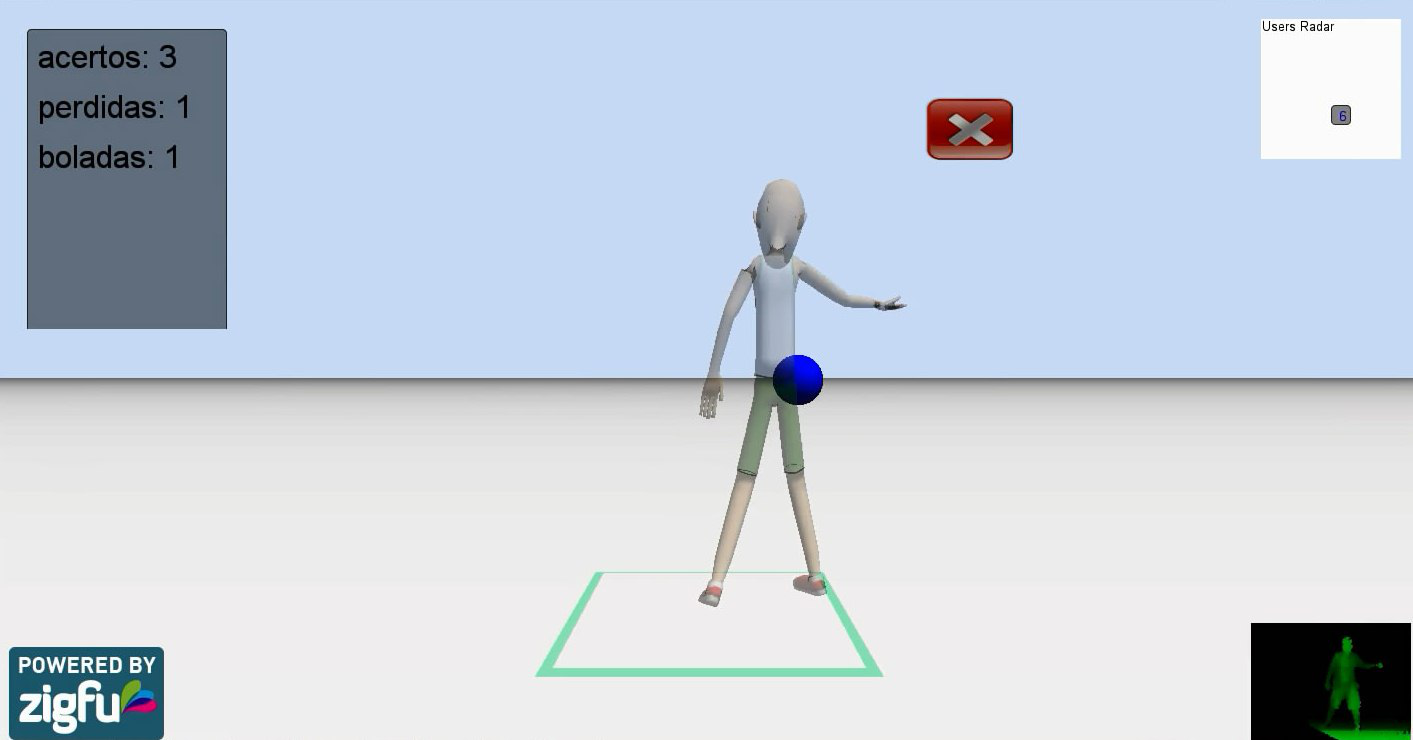
\includegraphics[width=.8\textwidth]{./img/catch-the-spheres.png}
     \caption{O jogo \emph{Catch the Spheres}}
     \label{img:catch}
\end{figure}

O mecanismo de aquisição e armazenamento dos sinais motores ([REQ-JOGUE-ME-05]) torna possível o envio de sinais motores de maneira colaborativa, usando um serviço responsável por receber e armazenar esses sinais. Na abordagem~\ac{jogue-me}, o servidor irá processar os sinais e transformá-los em informação para o profissional de saúde responsável pelo paciente.

\subsection{Arquitetura do \textit{JOGUE-ME Webservice}}
O mecanismo de aquisição e armazenamento dos sinais motores ([REQ-JOGUE-ME-05]) torna possível a análise dos dados motores do usuário no qual o jogo armazena as informações e as envia para o servidor de dados. 

O \textit{JOGUE-ME Webservice} é responsável por: criar usuário, receber dados motores, gerenciar arquivos exportá-los para o MATLAB~\cite{matlab2011} conforme a arquitetura descrita do Diagrama de Classes (Figura~\ref{fig:classd}).

\begin{figure}[!h]
     \centering
     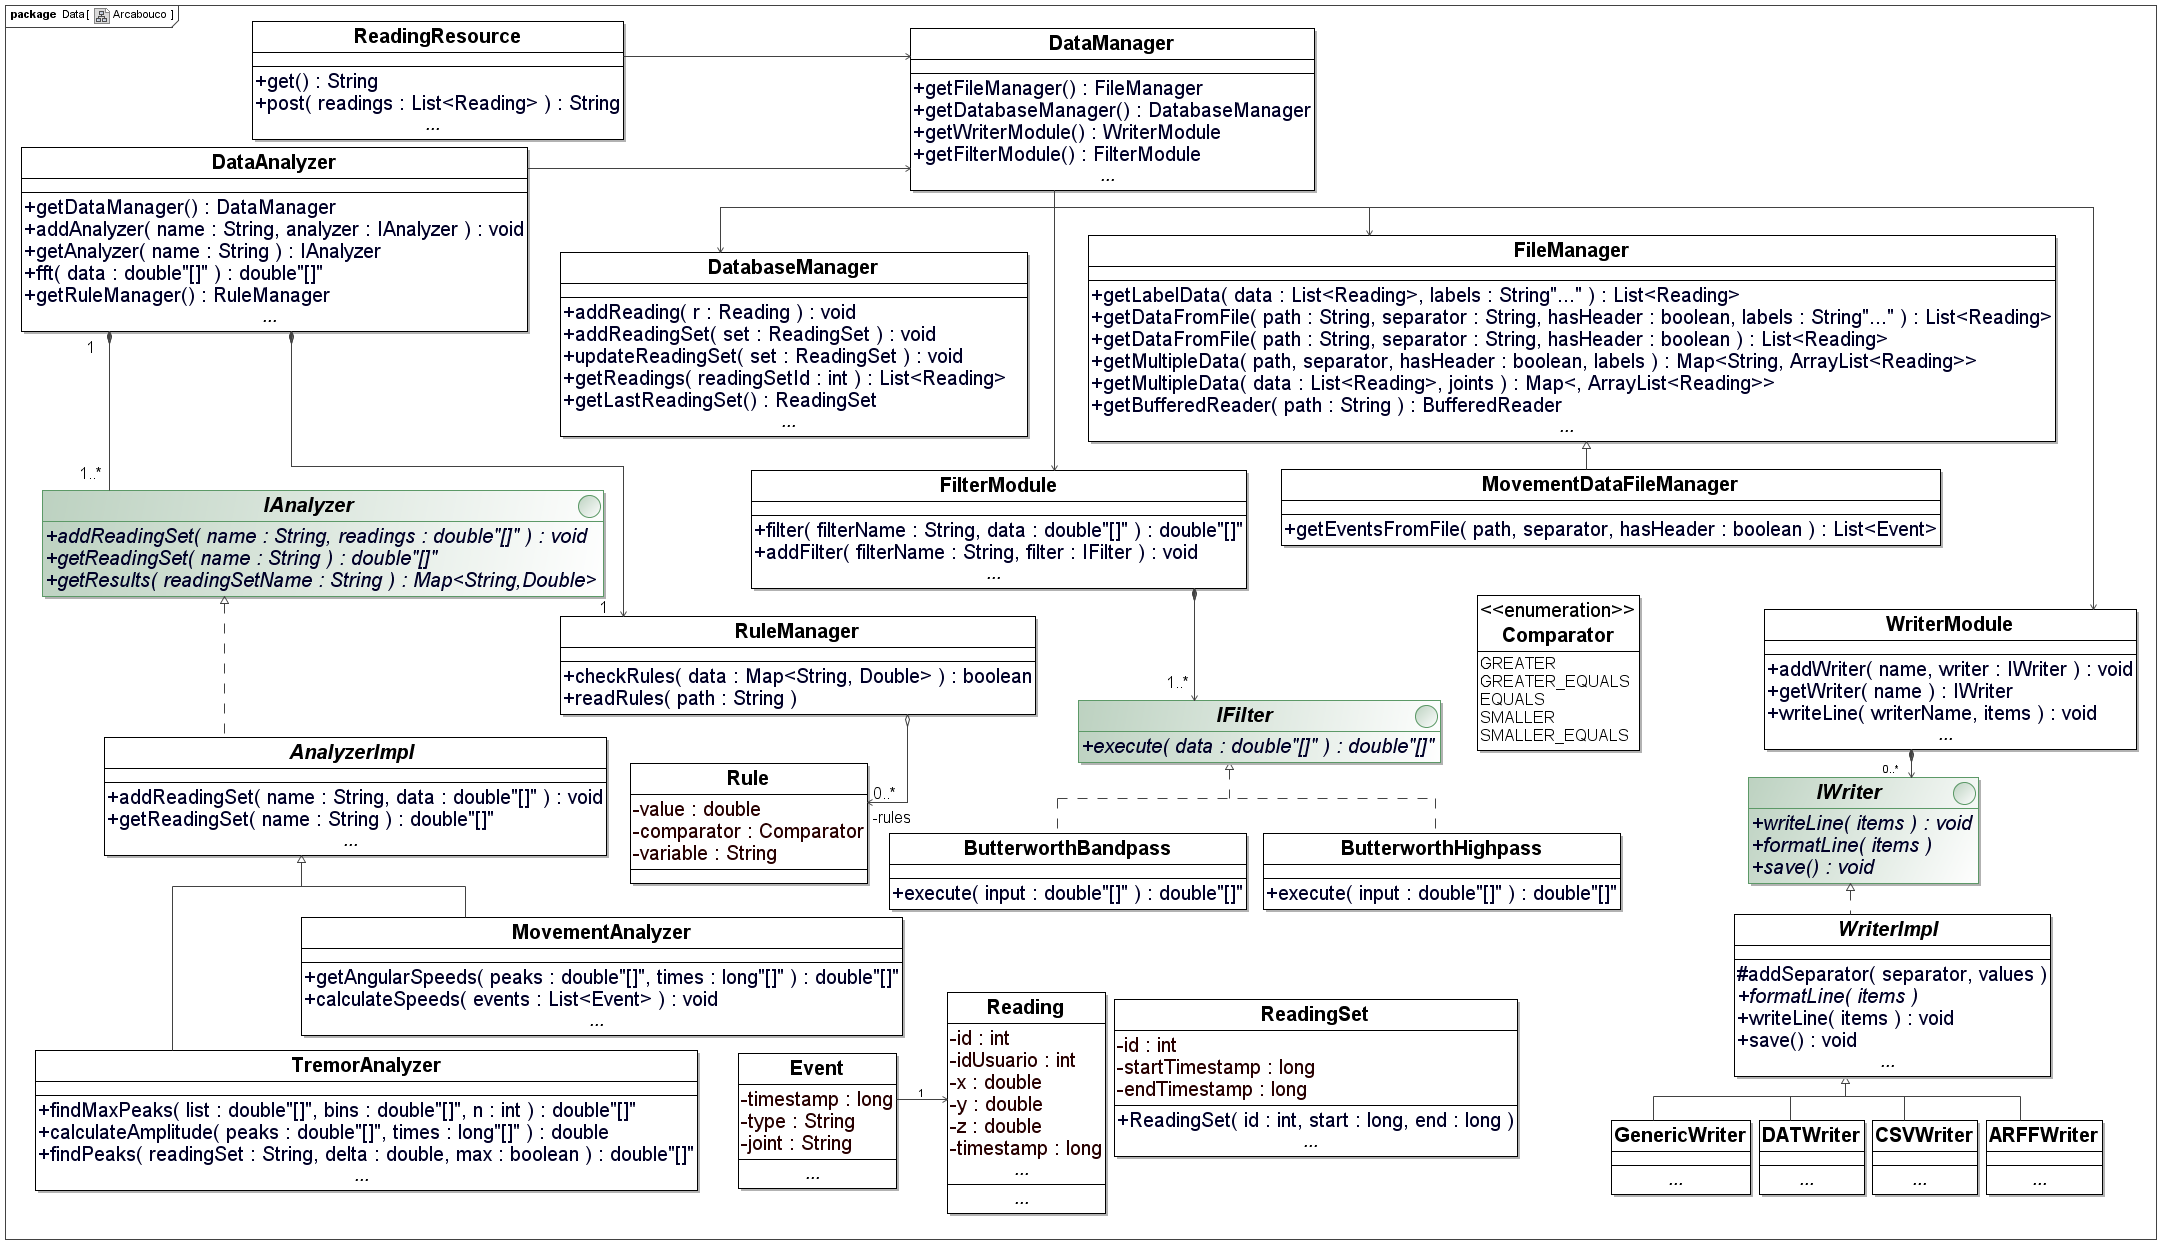
\includegraphics[width=1\textwidth]{./img/class_diagram.png}
     \caption[Diagrama de Classes do Serviço JOGUE-ME]{Diagrama de Classes do do Serviço JOGUE-ME}
     \label{fig:classd}
\end{figure}

O processo inicia com a aquisição dos dados dos sensores, que podem ser enviados para o \emph{webservice} e processados pela classe \texttt{ReadingResource} ou enviados por arquivos e processados pela classe \texttt{FileManager}, acessada através do \texttt{DataManager}. O \texttt{ReadingResource} envia os dados recebidos para o \texttt{DatabaseManager}, também acessado através do \texttt{DataManager}, para armazená-los no \emph{banco de dados} ~\cite{antonio2013}. Na Tabela~\ref{tab:operations}, ilustram-se as operações disponibilizadas pelo \textit{webservice} e um exemplo de como os dados devem ser estruturados para cada operação.

O envio dos dados dos usuários coletados com os dispositivos é feito através de uma requisição POST para o \textit{web service}. Os dados devem ser coletados durante uma sessão completa do jogo, que dura de alguns segundos a alguns minutos, para depois serem estruturados e enviados para o \textit{webservice}. O formato aceito pelas operações é o JSON (JavaScript Object Notation). 

\begin{table} 
\centering 
\caption{Operações disponibilizadas pelo \textit{web service}}
\begin{center}
    \begin{tabular}{ | l | c | l | }
        \hline
        Operação & Método & Exemplo \\ \hline
        cadastrarUsuario & POST & 
		\begin{minipage}{7cm}\begin{verbatim}
		
		{"id":2,"nome":"Ana",
		"masculino":false,
		"nascimento":"2012-11-28"}
		
		\end{verbatim}\end{minipage} \\ \hline
        obterToken & GET & - \\ \hline
        enviarDados & POST & 
		\begin{minipage}{7.5cm}\begin{verbatim}

		{"leitura":[{"id":0, 
		"idUsuario":1, "x":2.9097333, 
		"y":6.770132, "z":2.0355952, 
		"timestamp":1336134935706}, 
		{"id":0, "idUsuario":1, 
		"x":4.5565815, "y":4.9461093, 
		"z":1.4911331, 
		"timestamp":1336134935706}]}
		
		\end{verbatim}\end{minipage} \\ \hline
    \end{tabular}
\end{center}
\label{tab:operations}
\end{table}

\subsubsection{Gerenciador de Dados}
O \emph{Gerenciador de Dados} possui submódulos responsáveis por ler, separa e filtrar os dados, além do gerenciá-los usando um Banco de Dados para o armazenamento das informações motoras. A classe \texttt{DataManager} implementa as funcionalidades do \emph{Gerenciador de Dados}, referenciando os quatro módulos: \emph{Gerenciador de Arquivos}, \emph{Módulo de Escrita}, \emph{Módulo de Filtragem} e \emph{Gerenciador do Banco de Dados}. Estes módulos serão explicados nas subseções a seguir. A classe \texttt{DataManager} possui um construtor \texttt{DataManager(DatabaseManager, FileManager, WriterModule, FilterModule)}, que recebe como parâmetros os quatro módulos. Dessa forma, é possível aumentar a funcionalidade de cada um dos módulos estendendo suas respectivas classes por herança e adicionando a elas novos métodos. A classe \texttt{MovementDataFileManager}, tratada mais adiante, é um exemplo de extensão do \texttt{FileManager}.

O \emph{webservice}, implementado utilizou a biblioteca Jersey\footnote{Disponível em: http://jersey.java.net/}, que facilita o desenvolvimento de \textit{RESTful webservices}. As requisições são enviadas para serem processadas pela classe \texttt{ReadingResource}, que é um \textit{web resource}, uma entidade que recebe requisições HTTP e envia respostas. Esta classe possui dois métodos, o \texttt{get()} que trata requisições \emph{GET}, retornando o identificador do último conjunto de leituras para controle do armazenamento no banco de dados; e o método \texttt{post(List<Reading> readings)} processa os dados das leituras enviados através de requisições \emph{POST}, e convertidos de JSON para objetos Java pela biblioteca Jersey. A classe \texttt{ReadingResource} está acoplada à classe \texttt{DataManager} e, através dela, tem acesso ao \emph{Gerenciador do Banco de Dados}. O \emph{webservice} pode ser instalado em qualquer \textit{web container}, como o Apache Tomcat\footnote{Disponível em: http://tomcat.apache.org/} e o GlassFish\footnote{Disponível em: http://glassfish.
java.net/}.

\subsubsection{Gerenciador de Arquivos}

A classe \texttt{FileManager} implementa o módulo \emph{Gerenciador de Arquivos}, que processa as operações de abertura de arquivos de dados delegadas pelo \emph{Gerenciador de Dados}. Esse módulo processa os dados recebidos, armazenando-os em dados estruturados para serem processado posteriormente pelo \emph{Analisador de Dados}. O dado estruturado aceito pelo \emph{Analisador de Dados} é composto por um rótulo identificador do dado, uma marca de tempo com precisão de milissegundos, e coordenadas x, y e z, cujo significado depende do tipo de sensor que as gera.

Os métodos da classe \texttt{FileManager} são:
\begin{enumerate}
	\item \texttt{getLabelData(List<Reading> data, String... labels)} filtra os dados da lista de leituras \texttt{data}, retornando uma nova lista \texttt{List<Reading>} contendo apenas os dados com os rótulos definidos em \texttt{labels}.
	\item \texttt{getDataFromFile(String path, String separator, boolean hasHeader)} lê os dados de um arquivo localizado no caminho \texttt{path}, cujos dados estão separados pelo separador \texttt{separator} e definidos linha a linha. O parâmetro \texttt{hasHeader} indica se o método deve procurar por uma linha de cabeçalho na primeira linha do arquivo. Retorna uma \texttt{List<Reading>} com os dados.
	\item \label{getdatamethod} \texttt{getDataFromFile(String path, String separator, boolean hasHeader, String... labels)} estende a funcionalidade do método anterior, retornando uma \texttt{List<Reading>} com os dados que possuem os rótulos definidos em \texttt{labels}.
	\item \texttt{getMultipleData(String path, String separator, boolean hasHeader, String... labels)} possui a mesma função que o método~\ref{getdatamethod}, mas, diferente deste, retorna um \texttt{Map<String, List<Reading>>} onde cada chave do mapa é um rótulo e indexa uma lista de eventos identificados pelo rótulo.
	\item \texttt{getBufferedReader(String path)} retorna um \texttt{BufferedReader} para manipular o arquivo cujo caminho é especificado dem \texttt{path}.
\end{enumerate}

A classe \texttt{MovementDataFileManager} estende as funcionalidades do \texttt{FileManager}, adicionando um método para leitura de eventos oriundos de jogos. Os eventos marcam o início ou fim de um momento específico do jogo no qual o jogador estará executando um movimento que será enviado para análise.

\subsection{Módulo de Escrita}

O \emph{Módulo de Escrita} é implementado pela classe \texttt{WriterModule}, que é responsável pela saída dos dados processados pelo \emph{Analisador de Dados}. Os dados podem ser estruturados para serem mostrados em um programa de plotagem de gráficos, como o GNUPlot\footnote{Disponível em: http://www.gnuplot.info/}, ou para servirem como entrada para mecanismos de aprendizado de máquina. Os dados são escritos em CSV (\textit{Comma-separated Values}) ou em qualquer outro formato definido pelo usuário do arcabouço. O módulo de escrita também suporta a escrita de arquivos ARFF, para serem processados pelo Weka\footnote{Disponível em: http://www.cs.waikato.ac.nz/ml/weka/}. O \emph{Módulo de Escrita} é extensível para permitir a geração de um formato de arquivo específico. A criação de um novo arquivo de dados é feita através da extensão da classe \texttt{WriterImpl} pela classe que se está criando.

A interface \texttt{IWriter} define três métodos para manipular arquivos de dados:

\begin{enumerate}
	\item \label{formatlinemethod} \texttt{formatLine(Object... items)} formata os itens \texttt{items} adicionando separadores ou qualquer outra formatação adicional definida na classe específica de escrita que implementa \texttt{IWriter} ou estende \texttt{WriterImpl}.
	\item \texttt{writeLine(Object... items)} escreve uma nova linha no arquivo, seguindo a formatação definida pelo método~\ref{formatlinemethod}.
	\item \texttt{save()} fecha a \textit{stream} de escrita dedicada ao arquivo e salva o arquivo em disco.
\end{enumerate}

A classe \texttt{WriterImpl} implementa os métodos comuns a todas as classes de escrita, definidos pela interface \texttt{IWriter}, fornecendo um método adicional para incluir separadores entre os elementos de uma linha. Para definir um comportamento diferente daquele implementado por \texttt{WriterImpl}, deve-se implementar diretamente a interface \texttt{IWriter}.



%O \textit{JOGUE-ME Webservice} foi desenvolvido em colaboração com Antônio Santos Jr. em sua dissertação de mestrado ~\cite{antonio2013}. Do arcabouço do \textit{webservice} definido em seu trabalho, foram aproveitados os módulos de criação de usuário, recebimento de dados, gerenciador de arquivos e o módulo de escrita para gerar os arquivos a serem exportados e processados no MATLAB 2011 ~\cite{matlab2011} conforme a Arquitetura.

% \begin{figure}[!htb]
%      \centering
%      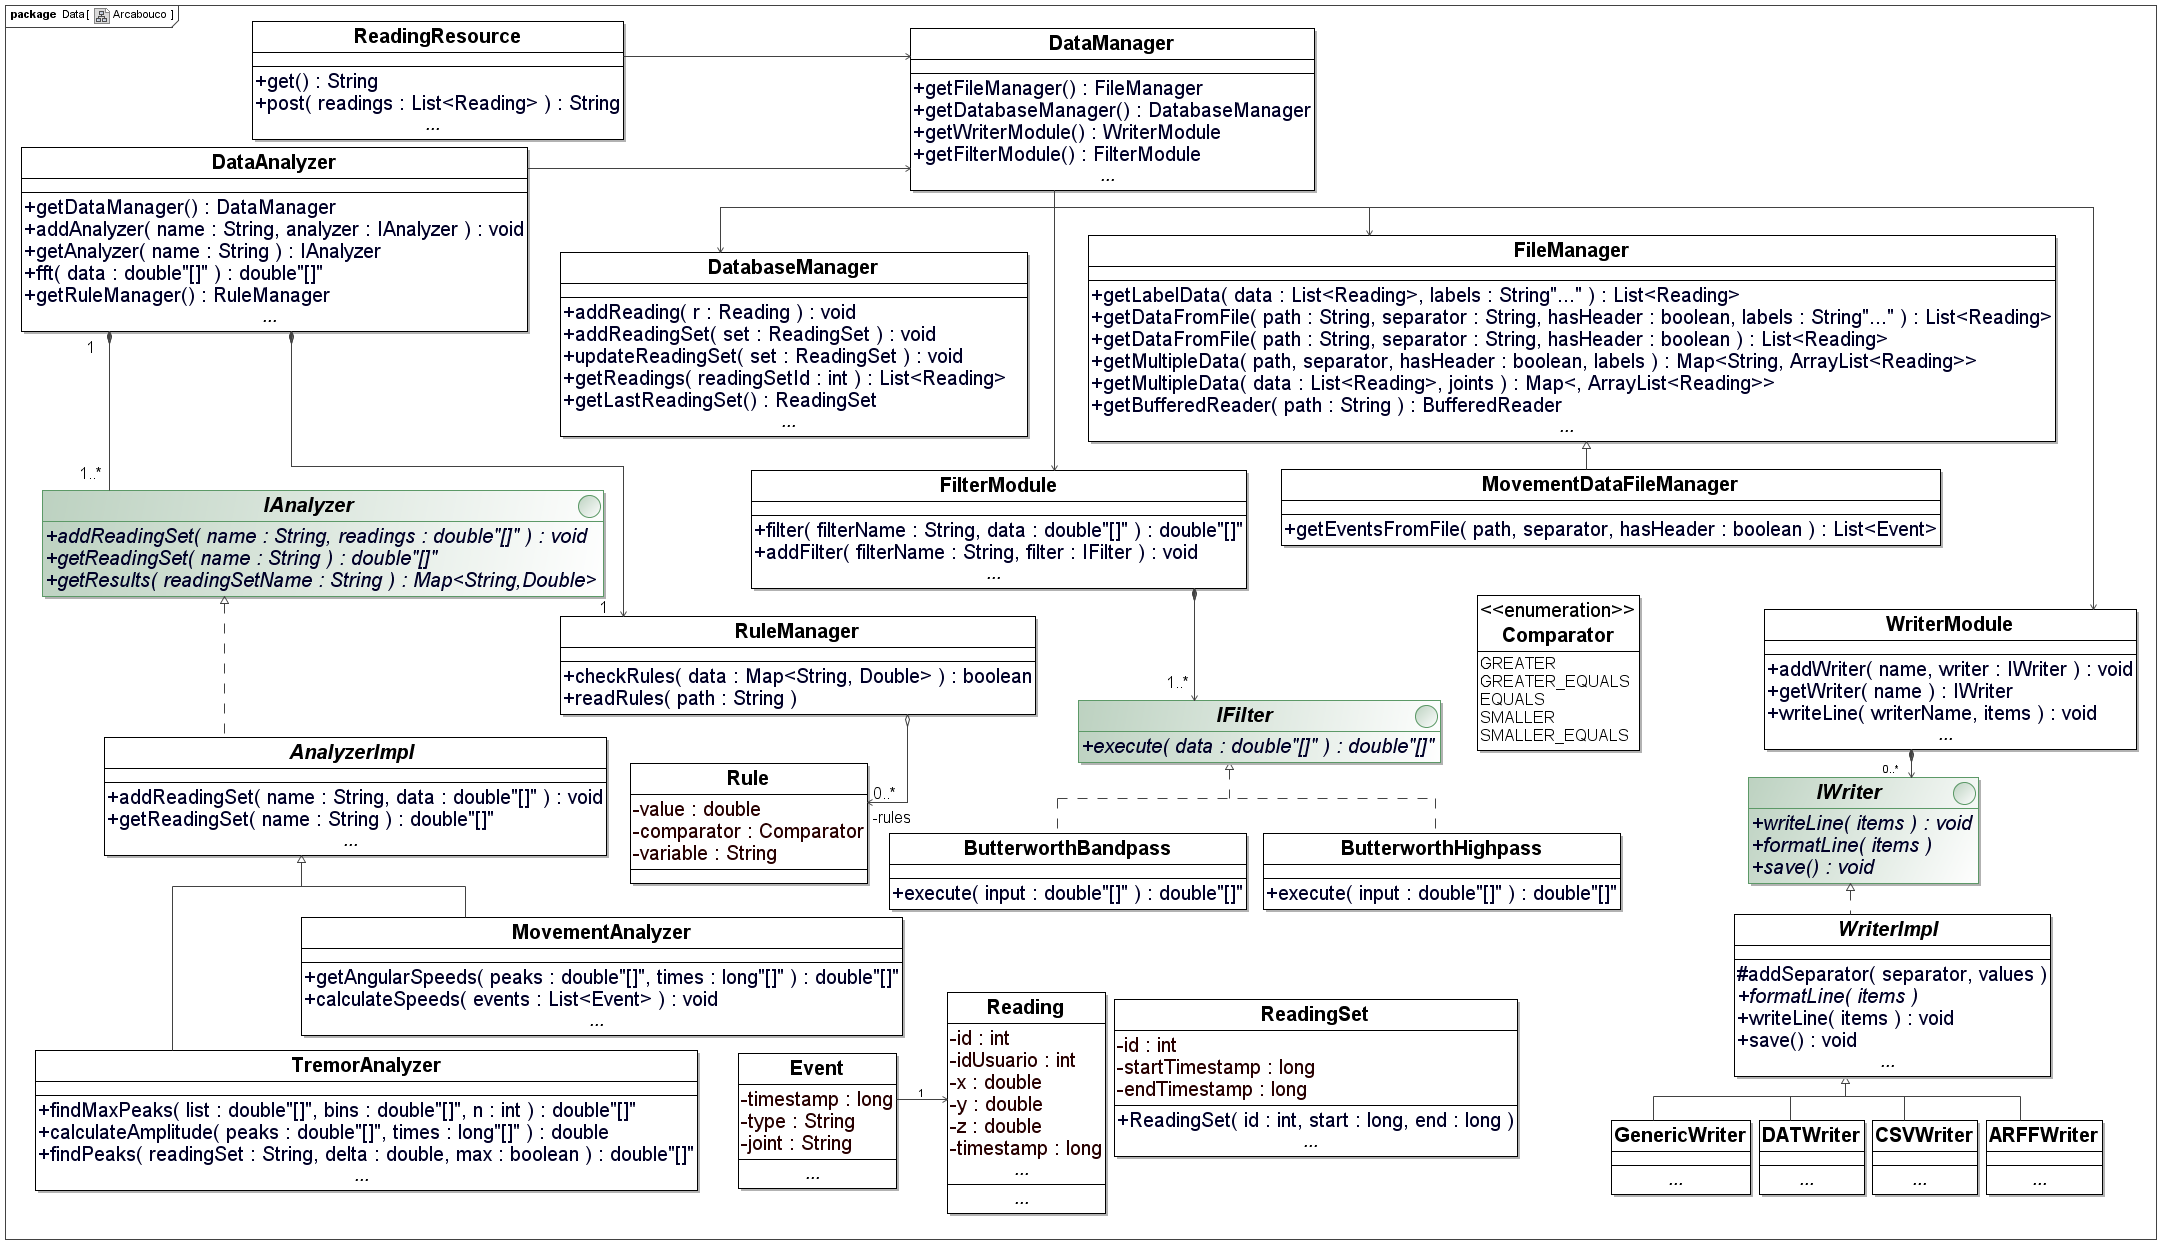
\includegraphics[width=1\textwidth]{./img/class_diagram.png}
%      \caption[Diagrama de Classes do Arcabouço]{Diagrama de Classes do Arcabouço ~\cite{antonio2013}}
%      \label{img:classd}
% \end{figure}

%O processo inicia com a aquisição dos dados dos sensores, que podem são enviados para o \emph{webservice} e processados pela classe \texttt{ReadingResource} ou enviados por arquivos e processados pela classe \texttt{FileManager}, acessada através do \texttt{DataManager}. O \texttt{ReadingResource} envia os dados recebidos para o \texttt{DatabaseManager}, também acessado através do \texttt{DataManager}, para armazená-los no \emph{banco de dados} ~\cite{antonio2013}. Na Tabela~\ref{tab:operations}, ilustram-se as operações disponibilizadas pelo \textit{webservice} e um exemplo de como os dados devem ser estruturados para cada operação.

%Os usuários enviam seus sinais, utilizando um cliente ~\ac{jogue-me} através de uma requisição \textit{POST}. Essa requisição é enviada no momento da finalização do jogo.
% 
% \begin{table} 
% \centering 
% \caption{Operações disponibilizadas pelo \textit{web service}}
% \begin{center}
%     \begin{tabular}{ | l | c | l | }
%         \hline
%         Operação & Método & Exemplo \\ \hline
%         cadastrarUsuario & POST & 
% 		\begin{minipage}{7cm}\begin{verbatim}
% 		
% 		{"id":2,"nome":"Ana",
% 		"masculino":false,
% 		"nascimento":"2012-11-28"}
% 		
% 		\end{verbatim}\end{minipage} \\ \hline
%         obterToken & GET & - \\ \hline
%         enviarDados & POST & 
% 		\begin{minipage}{7.5cm}\begin{verbatim}
% 
% 		{"leitura":[{"id":0, 
% 		"idUsuario":1, "x":2.9097333, 
% 		"y":6.770132, "z":2.0355952, 
% 		"timestamp":1336134935706}, 
% 		{"id":0, "idUsuario":1, 
% 		"x":4.5565815, "y":4.9461093, 
% 		"z":1.4911331, 
% 		"timestamp":1336134935706}]}
% 		
% 		\end{verbatim}\end{minipage} \\ \hline
%     \end{tabular}
% \end{center}
% \label{tab:operations}
% \end{table}

\section{Processador de Dados Biomecânicos}\label{sec:processador_bio}
Para transformar os sinais em informação, tanto para o profissional de saúde, quanto para máquinas de aprendizagem, é necessário fazer o processamento desse sinal. Neste trabalho, foi implementado o \textit{Processador de Dados Biomecânicos} em MATLAB 2011~\cite{matlab2011}. Este processador consiste de três passos: Identificação dos Ciclos, Extração de Características e Filtragem de Dados.

\subsection{Identificação dos Ciclos de Movimento} 
A identificação dos ciclos de movimento foi baseada na identificação de picos e vales do sinal motor, como explicado na Seção~\ref{section:identificao_ciclos}. 

Para implementar o mecanismo de detecção de ciclos, fez-se o uso da biblioteca \textit{Peak Detection in Matlab}~\cite{peakdetect}. Essa biblioteca possui uma função chamada \textit{peakdet()}, que recebe como parâmetros um vetor contendo o sinal a ser processado e um valor de limiar para remoção do ruído do sinal. A função retorna dois vetores: um possui os valores das máximas (picos) e o outro retorna os valores das mínimas (vales).

Usando a função \textit{peakdet()}, criou-se a função \textit{cycleperiodic()}, que tem o objetivo de identificar os ciclos periódicos de um sinal. Foram adicionados dois parâmetros a essa função, para justamente levar em consideração as amplitudes máximas e mínimas permitidas por este sinal.

%\begin{lstlisting}[frame=single, caption=Função de Ciclo Periódico]  % Start your code-block
%
%function [cycleIndex]=cycleperiodic(v, delta, maxAmplitude, minAmplitude)
%[peaks, valey] = peakdet(v, delta);
%j = 1;
%for (i=1:(size(valey,1)-1))    
    %initialIndex = valey(i,1);
    %endIndex = valey(i+1,1);
    %amplitude = endIndex - initialIndex;
    %if ((maxAmplitude >= amplitude) & (minAmplitude <= amplitude))
        %cycleIndex(j) = valey(i);
        %j = j +1;
    %end
%end
%\end{lstlisting}

De posse dos ciclos, pôde ser identificado quando começam e terminam os movimentos periódicos (Código Fonte~\ref{lst:identifyCycles}), como, por exemplo, os movimentos sucessivos de adução e abdução do braço (Seção ~\ref{fig:movabducaoaducao}). 

\begin{lstlisting}[frame=single, caption=Identificar Início e Tamanho do Movimento Periódico, label=lst:identifyCycles]  % Start your code-block

function [WindowBeginLeft, WindowLengthLeft, WindowBeginRight, WindowLengthRight] = identifyCycles(leftWristJoint, rightWristJoint)
    signalLeft = leftWristJoint(:,3);
    signalRight = rightWristJoint(:,3);

    cycleIndexLeft = cycleperiodic(signalLeft, 500, 200, 40);
    cycleIndexRight = cycleperiodic(signalRight, 500, 200, 40);

    WindowBeginLeft = cycleIndexLeft(1);
    WindowLengthLeft = cycleIndexLeft(size(cycleIndexLeft,2));
    WindowBeginRight = cycleIndexRight(1);
    WindowLengthRight = cycleIndexRight(size(cycleIndexRight,2));
\end{lstlisting}

\subsection{Extração das Características do Movimento}
Supondo que os ciclos de movimento foram identificados através da posição do punho, é necessário extrair as características do movimento. Para isso, o primeiro passo é calcular os ângulos relativos do movimento angular, usando os pontos das articulações, como pode ser visto no Código Fonte~\ref{lst:calculate_angle}. Então, a função \textit{ArmRelativeAngleTorso()} realiza o cálculo do produto escalar entre as três articulações.

\begin{lstlisting}[frame=single, caption=Calcular ângulos relativos do movimento, label=lst:calculate_angle]
leftShoulderJoint = leftShoulderJoint(WindowBeginLeft:WindowLengthLeft,:);
leftWristJoint = leftWristJoint(WindowBeginLeft:WindowLengthLeft,:);  
leftHipJoint = leftHipJoint(WindowBeginLeft:WindowLengthLeft,:);  

for (j=1:size(leftHipJoint,1))
leftArmAngle(j,1) = leftHipJoint(j,1);
        

leftArmAngle(j,2) = ArmRelativeAngleTorso(leftHipJoint,leftShoulderJoint,leftWristJoint, j);    
end
\end{lstlisting}

De posse do sinal dos ângulos relativos do movimento, são extraídos os picos e os vales desse sinal para calcularmos a velocidade angular do movimento de abdução e adução do braço (Código Fonte: ~\ref{lst:angular_velocity}).
    
\begin{lstlisting}[frame=single, caption=Calcular Velociodade Angular Adução e Abdução, label=lst:angular_velocity]	
distanceup = cycle(peak) - cycle(1);
amplitude(identifiedCycles,1) = cycle(peak);
    
timestampupsec = (abs(timestampcycle(1) - timestampcycle(peak)))/1000;
velocityUp(identifiedCycles,1) = distanceup/timestampupsec;

distancedown = abs(cycle(end) - cycle(peak));
timestampdownsec = (abs(timestampcycle(peak) - timestampcycle(end)))/1000;
velocityDown(identifiedCycles,1) = distancedown/timestampdownsec;
\end{lstlisting}	
		
\subsection{Filtro de Dados}
O filtro de dados remove os ciclos de movimento incompletos ou com problemas na aquisição dos dados, como explicado na Seção~\ref{section:filtro_dados}. Nessa etapa, os ciclos são normalizados, escalonados e rotulados por usuário. 
De posse de todos os dados, é calculado um vetor médio dos ciclos normalizados, para definir um limiar (\textit{threshold}) de remoção dos ciclos (Código Fonte:~\ref{code:filtercycles}).

	\begin{lstlisting}[frame=single, caption=Calcular Velociodade Angular Adução e Abdução, label=code:filtercycles]
function [ KinnectData, processedCycles, labels ] = filterCyclesAndLabels (T, labels, otherFeatures, scaledLength)

    normalization = T;
    for i=1:size(T,1)
       normalization(i,1:scaledLength) = T(i,1:scaledLength)./max(T(i,1:scaledLength));
       normalization(i,scaledLength+1:scaledLength*2) = T(i,scaledLength+1:scaledLength*2)./max(T(i,scaledLength+1:scaledLength*2));
       normalization(isnan(normalization(i,1:scaledLength*2))) = min(normalization(i,1:scaledLength*2));
    end
    
    normalization(isnan(normalization)) = 0;
    
    if(size(T,2) > scaledLength*2) 
       normalization(:,scaledLength*2 + 1:end) =  T(:,scaledLength*2+1 : end)./max(T(:,scaledLength*2 + 1:end));
    end
    
    threshold = 1;
    meanOfNormalization = mean(normalization);
    u = ones(size(normalization,1),1);
    filterTestVector = sum((normalization - (u*meanOfNormalization)).^2,2);
    filterVector = filterTestVector<threshold;
    
       
    KinnectData = [T(filterVector,:) otherFeatures(filterVector,:)];
    processedCycles = T(filterVector,:);
    labels = labels(filterVector,:);    
end
\end{lstlisting}	


\section{Classificador de Dados}
Para avaliar os requisitos de identificação dos sinais motores ([REQ-JOGUE-ME-06]), é necessário um teste com seres humanos, para avaliar a aquisição e a classificação dos sinais. A abordagem de classificação dos dados é baseada em máquinas de aprendizagem, como explicado na Seção~\ref{section:class_dados}. O Código Fonte~\ref{code:classification} demonstra como fazer a classificação dos dados utilizando o \textit{Matlab Statistics Toolbox}~\cite{matlab2011}, que possui um~\ac{svm} disponível em sua biblioteca.

Primeiramente, separa-se o grupo de treinamento para realizar a aprendizagem da máquina, utilizando o método \textit{svmtrain()}; depois utiliza-se o método \textit{svmclassify()} para predizer os valores usando esta máquina de aprendizagem; por fim, calculam-se as diferenças entre os valores reais. Então, é calculada a taxa de erro para avaliar o resultado do classificador.

\begin{lstlisting}[frame=single, caption=Uso de Máquina de Vetor de Suporte para Classificação dos Dados, label=code:classification]
realValues; %Classe Atual
SVMStruct = svmtrain(trainingData,trainningClassification,'Kernel_Function', 'linear',	'BoxConstraint', 0.10);
class = svmclassify(SVMStruct, testData, 'showplot',true); %Classe Preditiva
classificationRate = sum(class~=realValues);
errorRate = classificationRate/size(classereal,2);
\end{lstlisting}

%\section{Considerações Finais}
Neste capítulo foram apresentados os passos da implementação de um~\ac{jogue-me} para o monitoramento do sinal da bradicinesia presente no~\ac{dp}. Demonstramos na Seção~\ref{sec:processador_bio} o processador de dados biomecânicos implementado para identificar o sinal da bradicinesia~\cite{protpar010} presente no~\ac{dp}. Na Seção~\ref{sec:resultado_svm} do Capítulo~\ref{chap:avaliacao} serão demonstrados os experimentos realizados para validar esta arquitetura do~\ac{jogue-me}.

%Para reaplicar esta implementação em outros~\ac{sms}  Esta arquitetura pode ser reaplicada em outros contextos, mas como vimos na Seção